%%%%%%%%%%%%%%%%%%%%%%%%%%%%%%%%%%%%%%%%%%%%%%%%%%%%%%%%%%%%%%%%%%%%%%%%%%
%%%%%                         CHAPITRE 7                            %%%%%%
%%%%%%%%%%%%%%%%%%%%%%%%%%%%%%%%%%%%%%%%%%%%%%%%%%%%%%%%%%%%%%%%%%%%%%%%%%

\lhead[\fancyplain{}{\leftmark}]%Pour les pages paires \bfseries
      {\fancyplain{}{}} %Pour les pages impaires
\chead[\fancyplain{}{}]%
      {\fancyplain{}{}}
\rhead[\fancyplain{}{}]%Pour les pages paires 
      {\fancyplain{}{\rightmark}}%Pour les pages impaires \bfseries
\lfoot[\fancyplain{}{}]%
      {\fancyplain{}{}}
\cfoot[\fancyplain{}{\thepage}]%\bfseries
      {\fancyplain{}{\thepage}} %\bfseries
\rfoot[\fancyplain{}{}]%
     {\fancyplain{}{\scriptsize}}


%%%%%%%%%%%%%%%%%%%%%%%%%%%%%%%%%%%%%%%%%%%%%%%%%%%%%%%%%%%%%%%%%%%%%%%%%%
%%%%%                      Start part here                          %%%%%%
%%%%%%%%%%%%%%%%%%%%%%%%%%%%%%%%%%%%%%%%%%%%%%%%%%%%%%%%%%%%%%%%%%%%%%%%%%

\chapter{Application to BMX racing, jointly capturing pilot and bike}
\label{ch:7}

%==============================================================================	Résumé du chapitre

\begin{center}
\rule{0.7\linewidth}{.5pt}
\begin{minipage}{0.7\linewidth}
\smallskip

\textit{Numerous sports disciplines are practiced with special equipment, such as a board in skateboarding, a racket and a ball in tennis, or a bike in BMX racing. The interactions between the athlete and their gear are often important to retrieve. We analyzed BMX start sequences, by using OpenPose for 2D human pose estimation, and a custom trained DeepLabCut model for bike detection. We ran Pose2Sim on the joint {pilot+bike} 2D estimations, and performed 3D inverse kinematics on a custom OpenSim {pilot+bike} model. This showed that analyzing simultaneously the athlete and their equipment is possible, which provides additional perspectives for markerless sports motion analysis.\newline
See Figure~\ref{fig_visabstract5} for a visual abstract.
}

%\smallskip
\end{minipage}
\smallskip
\rule{0.7\linewidth}{.5pt}
\end{center}

\newpage

\minitoc

\vspace*{3cm}

\begin{figure}[hbtp]
	\centering
	\def\svgwidth{1\columnwidth}
	\fontsize{10pt}{10pt}\selectfont
	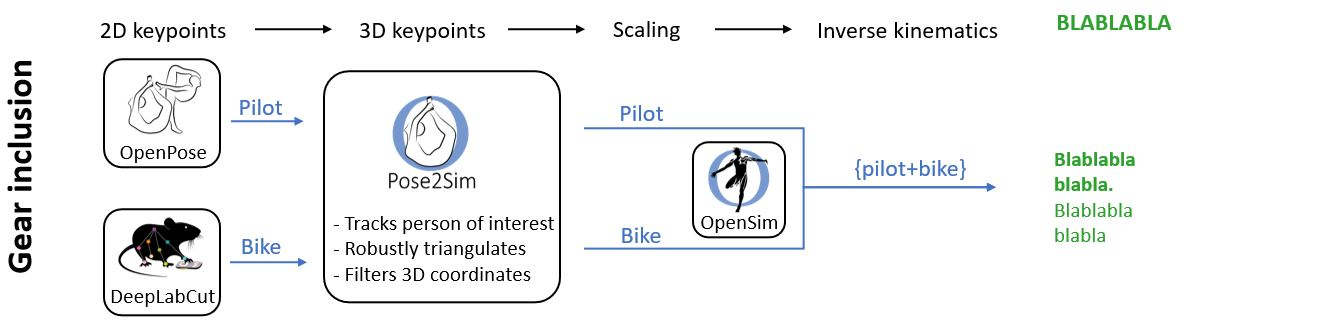
\includegraphics[width=\linewidth]{"../Intro/Figures/Fig_VisAbstract5.JPG"}
      \caption{Visual abstract for joint analysis of the athlete with OpenPose, and their equipment with DeepLabCut.}
	\label{fig_visabstract5}
\end{figure}

\newpage



Chap3:
On a different note, in a sports context, not only the human pose is of interest: sports gear can also be considerably important to detect, such as a ball \cite{Ghasemzadeh2021}, skis \cite{Ludwig2020}, or bike parts in the context of cycling (see Chapter 7 on \hyperref[ch:7]{Joint OpenPose and DeepLabCut detection}). This can help to analyze game dynamics, and to quantify posture cues related to a specific sports discipline. This can be done, for example, by separately process the video with OpenPose, as well as with a custom-trained DeepLabCut model. Resulting .trc coordinate files can be merged, and used in OpenSim. However, the DeeLabCut keypoints must be referenced on an OpenSim model, which may need to be crafted from scratch, such as a ball, skis, or bike, depending on the detected object.


\section{Introduction}
\subsection{The start in BMX racing}
\blindtext


\section{Methods}
\subsection{Material and protocol}
\blindtext

\subsection{Pilot inverse kinematics}
\blindtext

\subsection{Bike inverse kinematics}
\blindtext

\subsection{Joined pilot and bike inverse kinematics}
Marche pas avec nos qualités de vidéo : simulations

\blindtext


\section{Results}
\blindtext


\section{Discussion}
\subsection{On these data}
\blindtext

\subsection{Limits and perspectives}


Mathis2020 Principles, pitfalls and perspectives

% ajouter video de use on your own data
splashes, occlusions, distance, etc

Voir Protocole doc: % https://1drv.ms/w/s!AvGG4T_aAnWzmy4JuQph05pIphXX?e=0yjqbs
